% ================= SEKCJA 5 =================
\section{Diagram przypadkow uzycia}

W celu poprawy czytelnosci zamiast jednego rozbudowanego diagramu przygotowano cztery osobne diagramy przypadkow uzycia. Pierwszy przedstawia ogolny obraz systemu, natomiast kolejne trzy koncentruja sie na najwazniejszych obszarach funkcjonalnych aplikacji.

\subsection{Diagram ogolny systemu}

\begin{figure}[H]
    \centering
    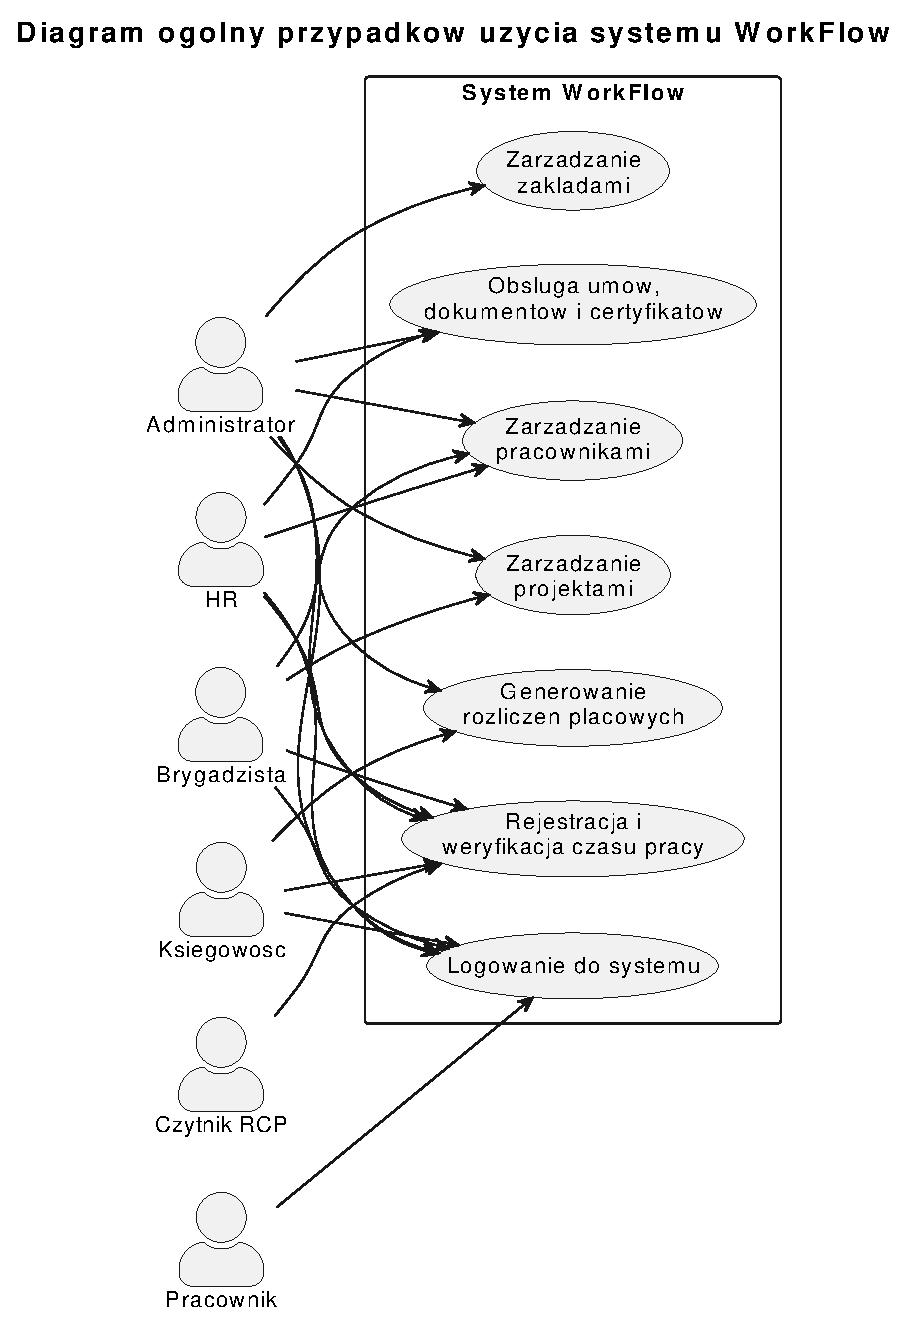
\includegraphics[width=\textwidth,height=0.82\textheight,keepaspectratio]{rys/plantuml-ogolny.pdf}
    \caption{Ogólny diagram przypadków użycia systemu \texttt{WorkFlow}}
    \label{fig:usecase-overall}
\end{figure}

\subsection{Modul kadrowy}

\begin{figure}[H]
    \centering
    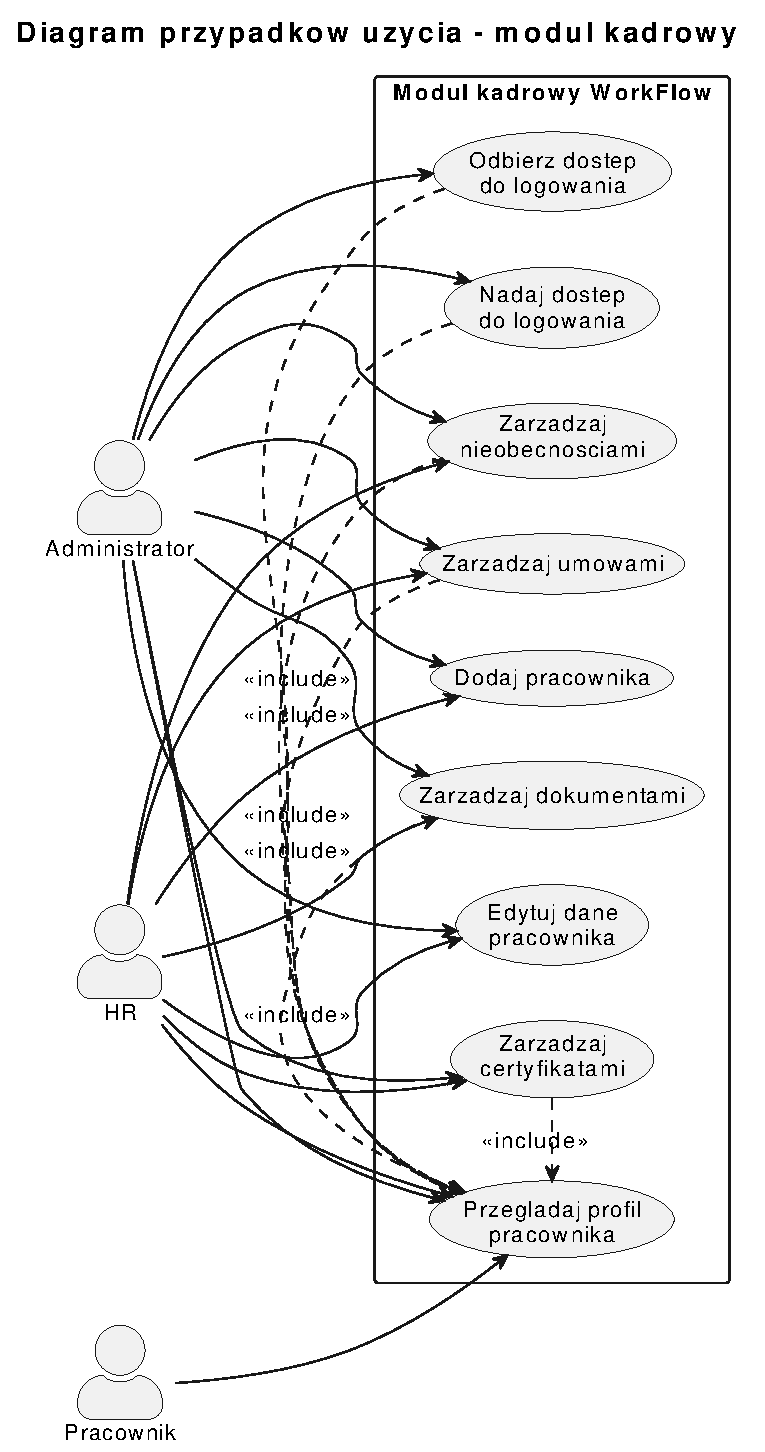
\includegraphics[width=\textwidth,height=0.82\textheight,keepaspectratio]{rys/plantuml-kadry.pdf}
    \caption{Diagram przypadków użycia dla modułu kadrowego}
    \label{fig:usecase-hr}
\end{figure}

\subsection{Czas pracy, RCP i rozliczenia}

\begin{figure}[H]
    \centering
    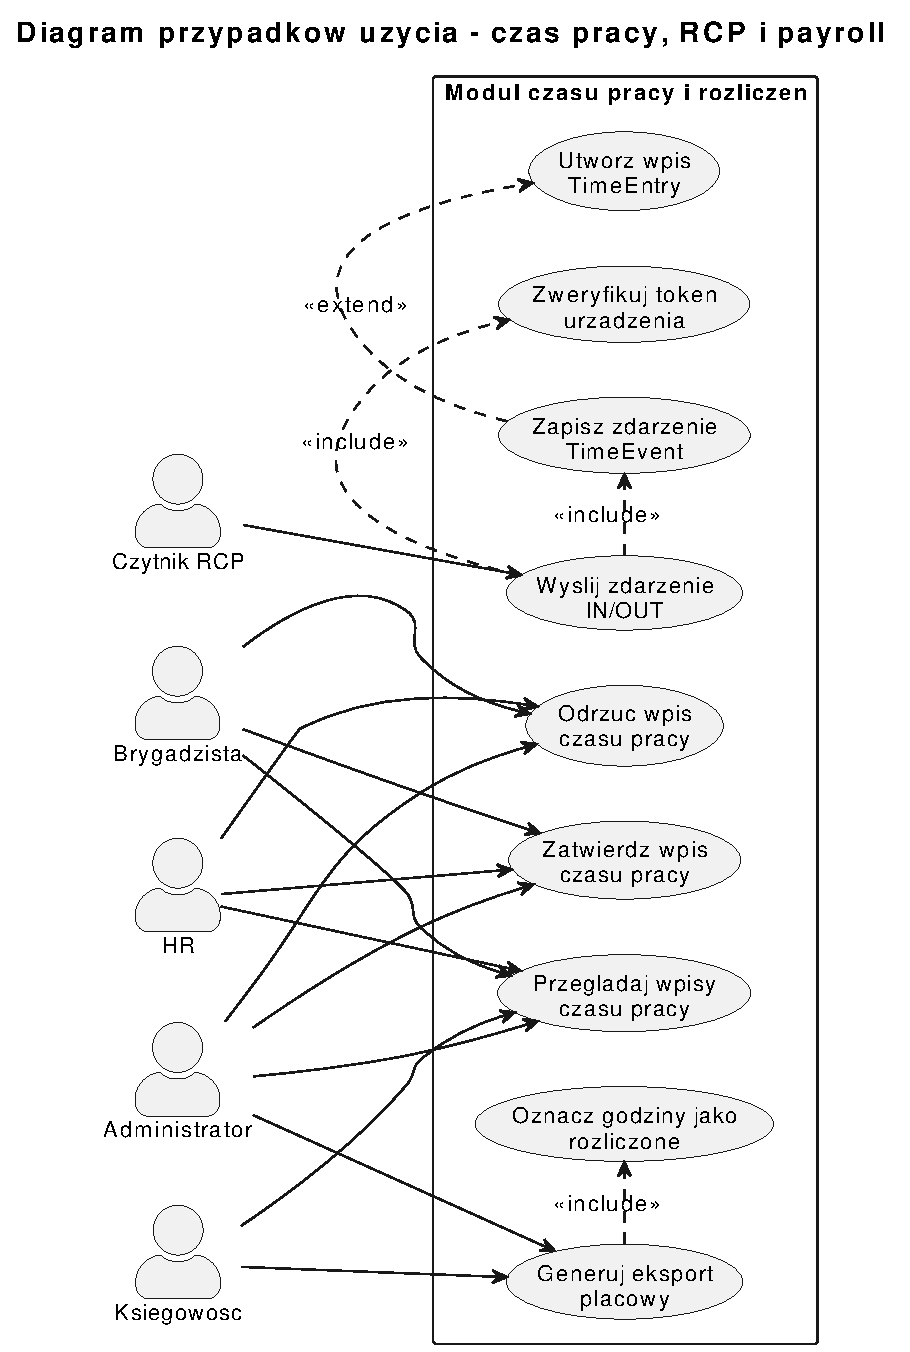
\includegraphics[width=\textwidth,height=0.82\textheight,keepaspectratio]{rys/plantuml-rcp-payroll.pdf}
    \caption{Diagram przypadków użycia dla rejestracji czasu pracy i rozliczeń}
    \label{fig:usecase-time}
\end{figure}

\subsection{Administracja i struktura organizacyjna}

\begin{figure}[H]
    \centering
    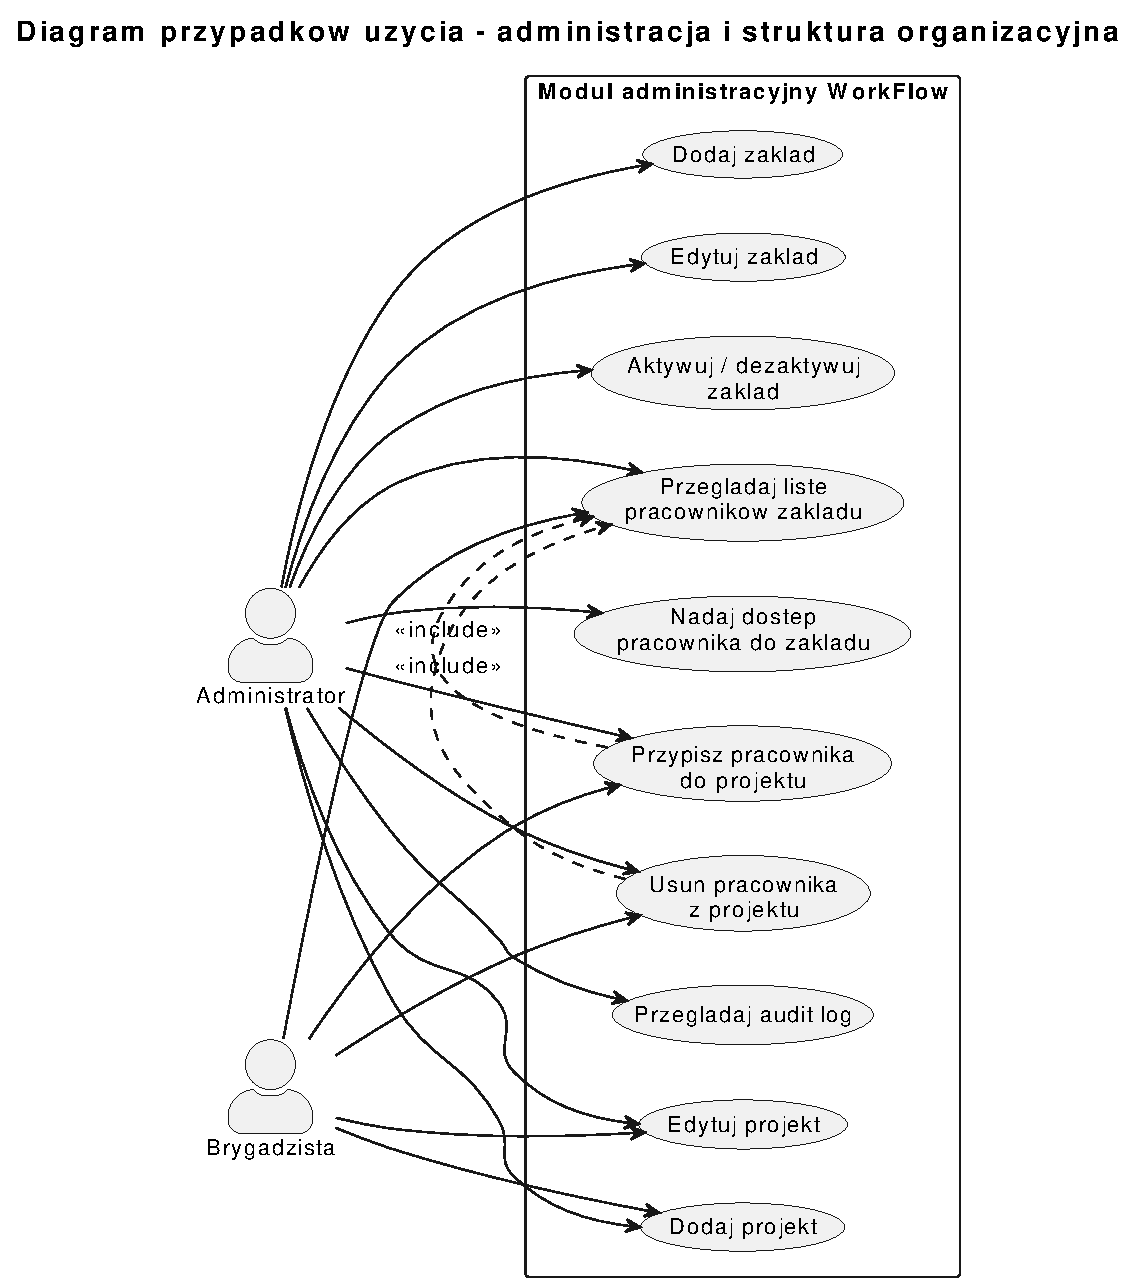
\includegraphics[width=\textwidth,height=0.82\textheight,keepaspectratio]{rys/plantuml-administracja.pdf}
    \caption{Diagram przypadków użycia dla administracji i zarządzania strukturą organizacyjną}
    \label{fig:usecase-admin}
\end{figure}

\subsection{Aktorzy systemu}

W systemie wyróżniono aktorów odpowiadających rolom użytkowników oraz jeden aktor techniczny reprezentujący czytnik RCP. Każdy aktor korzysta z innego zakresu funkcji, zgodnie z odpowiedzialnością w procesie obsługi pracowników, czasu pracy i dokumentacji.

\begin{itemize}
    \item \textbf{Administrator} -- użytkownik posiadający najszerszy zakres uprawnień. Odpowiada za ogólną konfigurację systemu, dostęp do zakładów, role użytkowników oraz kontrolę poprawności danych.
    \item \textbf{HR} -- użytkownik odpowiedzialny za obsługę danych kadrowych. Zarządza pracownikami, umowami, certyfikatami, dokumentami oraz nieobecnościami.
    \item \textbf{Księgowość} -- użytkownik korzystający z danych potrzebnych do rozliczeń. Pracuje głównie na zatwierdzonych wpisach czasu pracy i eksportach rozliczeniowych.
    \item \textbf{Brygadzista} -- użytkownik związany z pracą operacyjną. Ma dostęp do informacji dotyczących wybranych zakładów, projektów i pracowników.
    \item \textbf{Pracownik} -- podstawowa rola osoby znajdującej się w ewidencji systemu. W obecnym zakresie projektu rola ta pełni przede wszystkim funkcję danych pracowniczych, które są wykorzystywane przez inne moduły.
    \item \textbf{Czytnik RCP} -- aktor techniczny reprezentujący urządzenie wysyłające zdarzenia wejścia i wyjścia pracownika. Nie jest użytkownikiem interfejsu webowego, ale komunikuje się z backendem przez techniczny endpoint API.
\end{itemize}

\subsection{Zakres przypadków użycia}

Najważniejsze przypadki użycia systemu można podzielić na kilka grup funkcjonalnych:
\begin{itemize}
    \item \textbf{Uwierzytelnianie i dostęp} -- logowanie użytkownika, wylogowanie, sprawdzenie roli oraz zakresu dostępu do zakładów.
    \item \textbf{Zarządzanie strukturą organizacyjną} -- obsługa zakładów, przypisywanie pracowników do zakładów oraz nadawanie dostępu użytkownikom do wybranych jednostek.
    \item \textbf{Zarządzanie pracownikami} -- dodawanie, edycja, wyszukiwanie i przeglądanie pracowników oraz ich profili.
    \item \textbf{Zarządzanie projektami} -- tworzenie projektów, oznaczanie ich statusów oraz przypisywanie pracowników do projektów.
    \item \textbf{Rejestracja czasu pracy} -- odbieranie zdarzeń z czytników RCP, zapisywanie zdarzeń \texttt{IN}/\texttt{OUT} oraz tworzenie wpisów czasu pracy.
    \item \textbf{Obsługa dokumentacji kadrowej} -- obsługa umów, dokumentów, certyfikatów, badań, szkoleń i nieobecności.
    \item \textbf{Rozliczenia} -- przygotowanie danych rozliczeniowych oraz tworzenie eksportów payroll na podstawie zatwierdzonych wpisów czasu pracy.
    \item \textbf{Audyt} -- rejestrowanie wybranych operacji wykonywanych na danych systemu.
\end{itemize}

\subsection{Powiązanie ról z funkcjami}

Administrator posiada dostęp do największej liczby funkcji i odpowiada za konfigurację systemu oraz nadzór nad danymi. Rola HR koncentruje się na danych kadrowych, takich jak pracownicy, umowy, certyfikaty, nieobecności i dokumenty. Księgowość korzysta głównie z danych związanych z czasem pracy i rozliczeniami.

Brygadzista korzysta z danych operacyjnych, przede wszystkim z informacji o pracownikach, projektach i czasie pracy w ramach przypisanego obszaru. Pracownik jest podstawową encją systemu i może być powiązany z wieloma procesami, takimi jak przypisania do projektów, czas pracy, dokumenty, certyfikaty i nieobecności.

Czytnik RCP działa poza interfejsem użytkownika. Jego zadaniem jest przekazywanie zdarzeń technicznych do backendu. System na podstawie numeru seryjnego czytnika i identyfikatora karty RFID określa pracownika oraz projekt, którego dotyczy dane zdarzenie.

\subsection{Znaczenie diagramu dla projektu}

Diagram przypadków użycia porządkuje zakres funkcjonalny systemu i pokazuje, które role korzystają z poszczególnych modułów. Stanowi on punkt odniesienia dla dalszych scenariuszy użycia opisanych w kolejnym rozdziale.

Dzięki temu możliwe jest przejście od ogólnego obrazu funkcji systemu do konkretnych scenariuszy, takich jak logowanie użytkownika, zarządzanie profilem pracownika, rejestracja czasu pracy, kontrola ważności certyfikatów, obsługa nieobecności oraz przygotowanie danych rozliczeniowych.